%\documentclass[a4paper]{article}
%
%%% Language and font encodings
%\usepackage[english]{babel}
%\usepackage[utf8x]{inputenc}
%\usepackage[T1]{fontenc}
%\usepackage[noadjust]{cite}
%\usepackage{booktabs}
%\usepackage{subcaption}
%\renewcommand{\citedash}{--}  
%%% Sets page size and margins
%\usepackage[a4paper,top=3cm,bottom=2cm,left=3cm,right=3cm,marginparwidth=1.75cm]{geometry}
%
%%% Useful packages
%\usepackage{amsmath}
%\usepackage{url}
%\usepackage{graphicx}
%%\usepackage[colorinlistoftodos]{todonotes}
%\usepackage[colorlinks=true, allcolors=blue]{hyperref}
%
%\title{\textsc{Theia} DBD White Paper}
%%\author{T. Klosterman, V. Lozza, A. Mastbaum}
%
%\begin{document}
%\maketitle

%\section{Introduction}
The \textsc{Theia} search for neutrinoless double beta decay (NLDBD) aims for
sensitivity to the non-degenerate normal hierarchy parameter space
within the canonical framework of light Majorana neutrino exchange and
three-neutrino mixing, at the level of $m_{\beta\beta}\sim5$ meV.
This is achieved through the loading of a very large
mass of a NLDBD candidate isotope into an ultra-pure liquid scintillator
target, together with coincidence and topological particle identification
techniques.

\subsubsection{Detector Configuration}

For the present studies, we model the detector as a cylinder with a 20\,m fiducial radius and a 40\,m height, for a total fiducial mass of 50\,kt. The detector is assumed to be located in the Homestake mine, at a depth of 4300\,m.w.e. The double-beta decay isotope under investigation is loaded into a nylon balloon of 435\,$\mu$m thickness and 8\,m radius, filled with ultra-pure liquid scintillator (LAB + 2\,g/l PPO for a density of 0.86 g/cm$^3$). The volume outside the balloon is filled with a WbLS (10\% LAB-PPO and 90\% water). We investigate two major loading cases: 3\% enriched Xenon (89.5\% in $^{136}$Xe) and 5\% natural Tellurium (34.1\% in $^{130}$Te).

The optical properties of the unloaded LAB+PPO cocktail have been measured by the SNO+ collaboration, while those of the WbLS are obtained by weighting contributions of the LAB+PPO and water, and are consistent with benchtop measurements. As a baseline, an average light yield of 1200 PMT hits per deposited MeV is assumed (corresponding to about 3\%/$\sqrt(E)$ energy resolution). This value includes the reduction in the light yield due to the addition of the isotope, estimated to be around 30\% at 5\%, or higher, loadings. For the specific case of Xe loaded scintillator, the used light yield is likely an underestimation as the KamLAND-Zen experiment predicts a reduction of only 15\% at the reached 3\% loading, corresponding to 1530 Nhits/MeV \cite{KZ-2011}. Figure \ref{fig:scale-ly} shows the impact of the light yield on the THEIA sensitivity.
Simulations are obtained with the Geant4-based RAT-PAC software package \footnote{\url{https://github.com/rat-pac/rat-pac}}, part of the radioactive decays are simulated using the Decay0 code \cite{decay0}. Reconstructed energy is approximated by assuming the Poisson limit of
photon counting: the true deposited energy, accounting for quenching, is smeared out by a Gaussian resolution function corresponding to the light
yield.

\subsubsection{Backgrounds}

\begin{table}[t]
\centering
\scalebox{0.9}{
\begin{tabular}{lcccc}
\toprule
{\bf Source} & {\bf Target level} & {\bf Expected events/y}   & \multicolumn{2}{c}{\bf Events/ROI$\cdot$y} \\
& & & 5\% $^{nat}$Te  & 3\% $^{enr}$Xe  \\
\midrule
Balloon $^{10}$C  & & 500 &  2.5       & 2.5\\
$^{8}$B neutrinos (normalization from \cite{SNO_3ph}) &  & 2950   & 13.8      & 13.8  \\
$^{130}$I (Te target)  &  & 155  (30 from $^{8}$B) & 8.3 & - \\
%$^{136}$Cs (Xe target) &   & 47 (6 from $^{8}$B)   & &\\
$^{136}$Cs ($^\mathrm{enr}$Xe target) & & 478 (68 from $^{8}$B) & -&0.06\\
2$\nu\beta\beta$ (Te target, T$_{1/2}$ from \cite{Cuore017}) &   & 1.2$\times$10$^{8}$  & 8.0       &  -\\  
%2$\nu\beta\beta$ (Xe target,  T$_{1/2}$ from \cite{gando16, exo14})  & & 7.0$\times$10$^{6}$  & & \\  
2$\nu\beta\beta$ ($^\mathrm{enr}$Xe target, T$_{1/2}$ from \cite{gando16, exo14}) &  &  7.1$\times$10$^{7}$  &   -    & 3.8  \\  
Liquid scintillator & $^{214}$Bi: $10^{-17}$ g$_{U}$/g  & 7300 & 0.4        & 0.4\\
   & $^{208}$Tl: $10^{-17}$ g$_{Th}$/g  & 870  & -& -\\
Nylon Vessel  \cite{radiopurityorg, kamLAND_Zen}  & $^{214}$Bi: $<1.1\times10^{-12}$ g$_{U}$/g & 1.2$\times$10$^{5}$   & 2.4       & 2.7   \\
 & $^{208}$Tl: $<1.6\times10^{-12}$ g$_{Th}$/g   & 2.1$\times$10$^{4}$  & 0.03       & 0.01  \\
%PMTs  & $^{214}$Bi: $10^{-6}$ g$_{U}/$PMT  &  &&  \\
 %& $^{208}$Tl: $10^{-6}$ g$_{Th}/$PMT  & && \\
% {\bf Total}      &&         & 35.5      & 23.5      \\
\bottomrule
\end{tabular}}
\caption{Dominant background sources expected for the NLDBD search in \textsc{Theia}. The assumed loadings are 3\% for Xe, for a $^{136}$Xe mass of 49.5\,t, and 5\% for Te, for a $^{130}$Te mass of  31.4\,t. The events in the ROI/yr are given for a fiducial volume of 7\,m and an symmetric energy range around the Q-value of the reaction (\textit{see text}). A rejection factor of 92.5\% is applied to $^{10}$C, of 99.9\% to $^{214}$Bi, of 50\% to the balloon backgrounds, and of 50\% to the $^8$B solar neutrinos.}
\label{tab::bckg}
\end{table}

The main sources of background included in the this analysis are summarized in Table \ref{tab::bckg} and described below:

\begin{description}
\item[Double Beta Decay] This irreducible background is due to the $2\nu\beta\beta$ decays of $^{130}$Te or $^{136}$Xe. Due to the steeply-falling
spectrum, the number of events falling in the ROI depends strongly on the energy resolution.
\item[Cosmogenic Production] These backgrounds are due to activation of nuclei by muons (during data taking) or protons and neutrons (during material production and handling at Earth's surface). The neutron and proton production's rates in Xe and Te has been investigated by several authors \cite{mei09, baudis15, zhang16, norm05, bard97, wang15, lozza15}. Among the most important nuclides there are $^{60}$Co ($Q=2.8$ MeV, $T_{1/2}=5.27$ y) and $^{110m}$Ag ($Q=3.1$ MeV, $T_{1/2}=250$ d). Mitigation of these background sources requires minimal exposure at sea level, a deep underground cool-down period, chemical purification processes \cite{snop16}, and, to limit the in-situ production during data taking, the use of a water shield. In these studies, it is assumed that proper measures are taken to handle the target material, reducing the background to a negligible level. For what concerns the in-situ muon induced background, the most dangerous nuclide for the NLDBD study is $^{10}$C ($Q=3.65$ MeV, $T_{1/2}=19.3$ s) produced by muon interaction with the carbon atoms of the liquid scintillator. The estimated event's rate is about 300 events/kt/yr \cite{hagn00} for a muon flux of $4.2\times10^{-9}$ cm$^{-2}$ s$^{-1}$ and an average muon energy of 293\,GeV \cite{mei06}. A reduction of 92.5\% of the $^{10}$C background has been demostrated by Borexino \cite{bxo2013}, using a three-fold coincidence technique\cite{galb05, gando16}.
\item[Solar Neutrinos] $^{8}$B solar neutrino elastic scattering in the target material results in a background that is approximately flat across the NLDBD energy region of interest. These events can potentially be reduced using Cherenkov light to determine the direction with respect to the Sun and, possibly, separate one- and two-ring topologies, on a statistical basis, if not event-by-event. Figure \ref{fig:scale-b8} shows the sensitivity scaling with solar neutrino event's reduction.
Another background induced by solar neutrinos (mainly $^{8}$B and $^{7}$Be) are high Q-value nuclides produced by charged current interaction with $^{130}$Te and $^{136}$Xe \cite{eijiri14, eijiri17}. Due to their long half life, a tagging technique based on a delayed coincidence is expected to have a small efficiency. 
\item[Internal Contamination:] $^{214}$Bi ($Q=3.27$ MeV, U-chain) and $^{208}$Tl ($Q=5$ MeV, Th-chain) decays can fall in the energy window used for the NLDBD studies. The targeted scintillator cocktail purity for the \textsc{Theia} experiment is 10$^{-17}$ g/g in both U and Th. Liquid scintillator purities better than $\times$ 10$^{-18}$ g/g in U and Th have been obtained in the Phase-II of Borexino \cite{bxo16}, while KamLAND-Zen, has reached a cleanliness of the order of $\times$ 10$^{-16}$ g/g U for the 3\% loaded case \cite{gando13}. The targeted purity is considered achievable by improving the target material purification technique, i.e the purity grade of the chemicals used to process the tellurium. In addition delayed coincidence techniques can further reduce the number of $^{214}$Bi decays falling in the ROI. A rejection better than 99.95\% for the $^{214}$BiPo in the ROI has been shown by the KamLAND-Zen experiment \cite{KD-Zen}, while Monte Carlo studies for the SNO+ experiment show that the rejection in the double-beta decay region can be as high as 99.99\% \cite{snop16}. For the aimed target purity, it is required that the $^{214}$Bi is further reduced by 99.9\%. Larger reduction factors have a minimum effect on the overall sensitivity.
\item[External Sources:] Decays from U and Th-chain impurities present in the balloon material, the external water-based liquid scintillator, the
shielding water, and in the PMTs also contribute to the background. External background events can be reduced using a fiducial volume cut, and hit time information. In the following study a rejection factor of 50\%, on the top of the fiducial volume, is assumed. However, a smaller reduction factor won't affect the sensitivity.
\end{description}

\subsubsection{NLDBD Sensitivity: Counting Analysis}\label{sec::sensitivity}

To estimate the sensitivity, a single-bin counting analysis is employed. Since all backgrounds do not scale with isotope mass (e.g. solar neutrinos
and external $\gamma$ backgrounds), we use the Monte Carlo to evaluate the background expectation, establish a confidence region using the Feldman-Cousins frequentist approach, and derive an expected limit on the NLDBD half life:
\begin{equation}
\label{eq:sens}
\widehat{T}_{1/2}^{0\nu\beta\beta}(\alpha) = 
\frac{N\cdot \epsilon \cdot t \cdot \ln 2}{\mathrm{FC}(n=b, b; \alpha)}
%\widehat{T}_{1/2}^{0\nu\beta\beta}(\alpha) = \left\langle
%\frac{n\cdot \epsilon \cdot t \cdot \ln 2}{\mathrm{FC}(N, b; \alpha)}
%\right\rangle_{n=\mathrm{Pois}(b)}
\end{equation}
where $N$ is the number of atoms of active NLDBD isotope, $\epsilon$ is the efficiency, $t$ the live time, and $b$ the expected background.
`FC' refers to a Feldman-Cousins interval at confidence level $\alpha$.

The expected event rates per year for a $^\mathrm{nat}$Te or $^\mathrm{enr}$Xe loaded \textsc{Theia} detector are given in Table \ref{tab::bckg}, for a fiducial volume is 7\,m (67\%) and an asymmetric energy region,  from $-\sigma/2 \to 2\sigma$, to maximize signal acceptance ($\epsilon=66.9$\%) while removing much of the steeply-falling two-neutrino DBD background spectrum. Figure \ref{fig:spectrum-plots} shows the background spectra near the endpoint in the Te (Figure \ref{fig:spectrum-te}) and Xe (Figure \ref{fig:spectrum-xe}) cases.

The expected sensitivity (90\% CL sensitivity), using phase space factors from \cite{2012PhRvC..85c4316K} and matrix element from \cite{Barea:2013wb} (g$_{A}$=1.269) is:
\begin{eqnarray*}
\mathrm{\bf Te:}~~
  T_{1/2}^{0\nu\beta\beta} > 1.5\times10^{28}~\mathrm{y},~
  m_{\beta\beta} < 5.4~\mathrm{meV}\\
  \mathrm{\bf Xe:}~~
  T_{1/2}^{0\nu\beta\beta} > 2.7\times10^{28}~\mathrm{y},~
  m_{\beta\beta} < 4.8~\mathrm{meV}
\end{eqnarray*}


%\begin{table}
%\centering
%\begin{tabular}{ccc}
%\toprule
%                          & \multicolumn{2}{c}{\bf Events/ROI$\cdot$y} \\
%{\bf Signal}              & Te Loading & $^{enr}$Xe Loading \\
%Loaded isotope mass [t] & 31.4 & 49.5 \\
%\midrule
%$0\nu\beta\beta$ (10 meV) & 108.9       & 116.4      \\
%\midrule
%$2\nu\beta\beta$          & 80.0       & 38.2       \\
%$^8$B Solar ES  (50\%)           & 138.5      & 138.4      \\
%$^{10}$C  (92.5\%)                & 24.6       & 25.4       \\
%$^{130}$I                 & 80.5       & ---        \\
%$^{130m}$I                & 2.9        & ---        \\
%$^{136}$Cs                & ---        & 0.57       \\
%$^{208}$Tl                & 0.02       & 0.002      \\
%$^{214}$Bi  (99.9\%)               & 4.0        & 4.4        \\
%Balloon $^{214}$Bi  (50\%)       & 24.0       & 27.4       \\
%Balloon $^{208}$Tl  (50\%)      & 0.25       & 0.14       \\
%\midrule
%{\bf Total}               & 354.8      & 234.5      \\
%\bottomrule
%\end{tabular}
%\caption{Expected background counts per year in the ROI. In parenthesis is shown the reduction factor applied.}
%\label{tab:counts}
%\end{table}

\begin{figure}[!h]
\centering
\begin{subfigure}[b]{0.35\textwidth}
 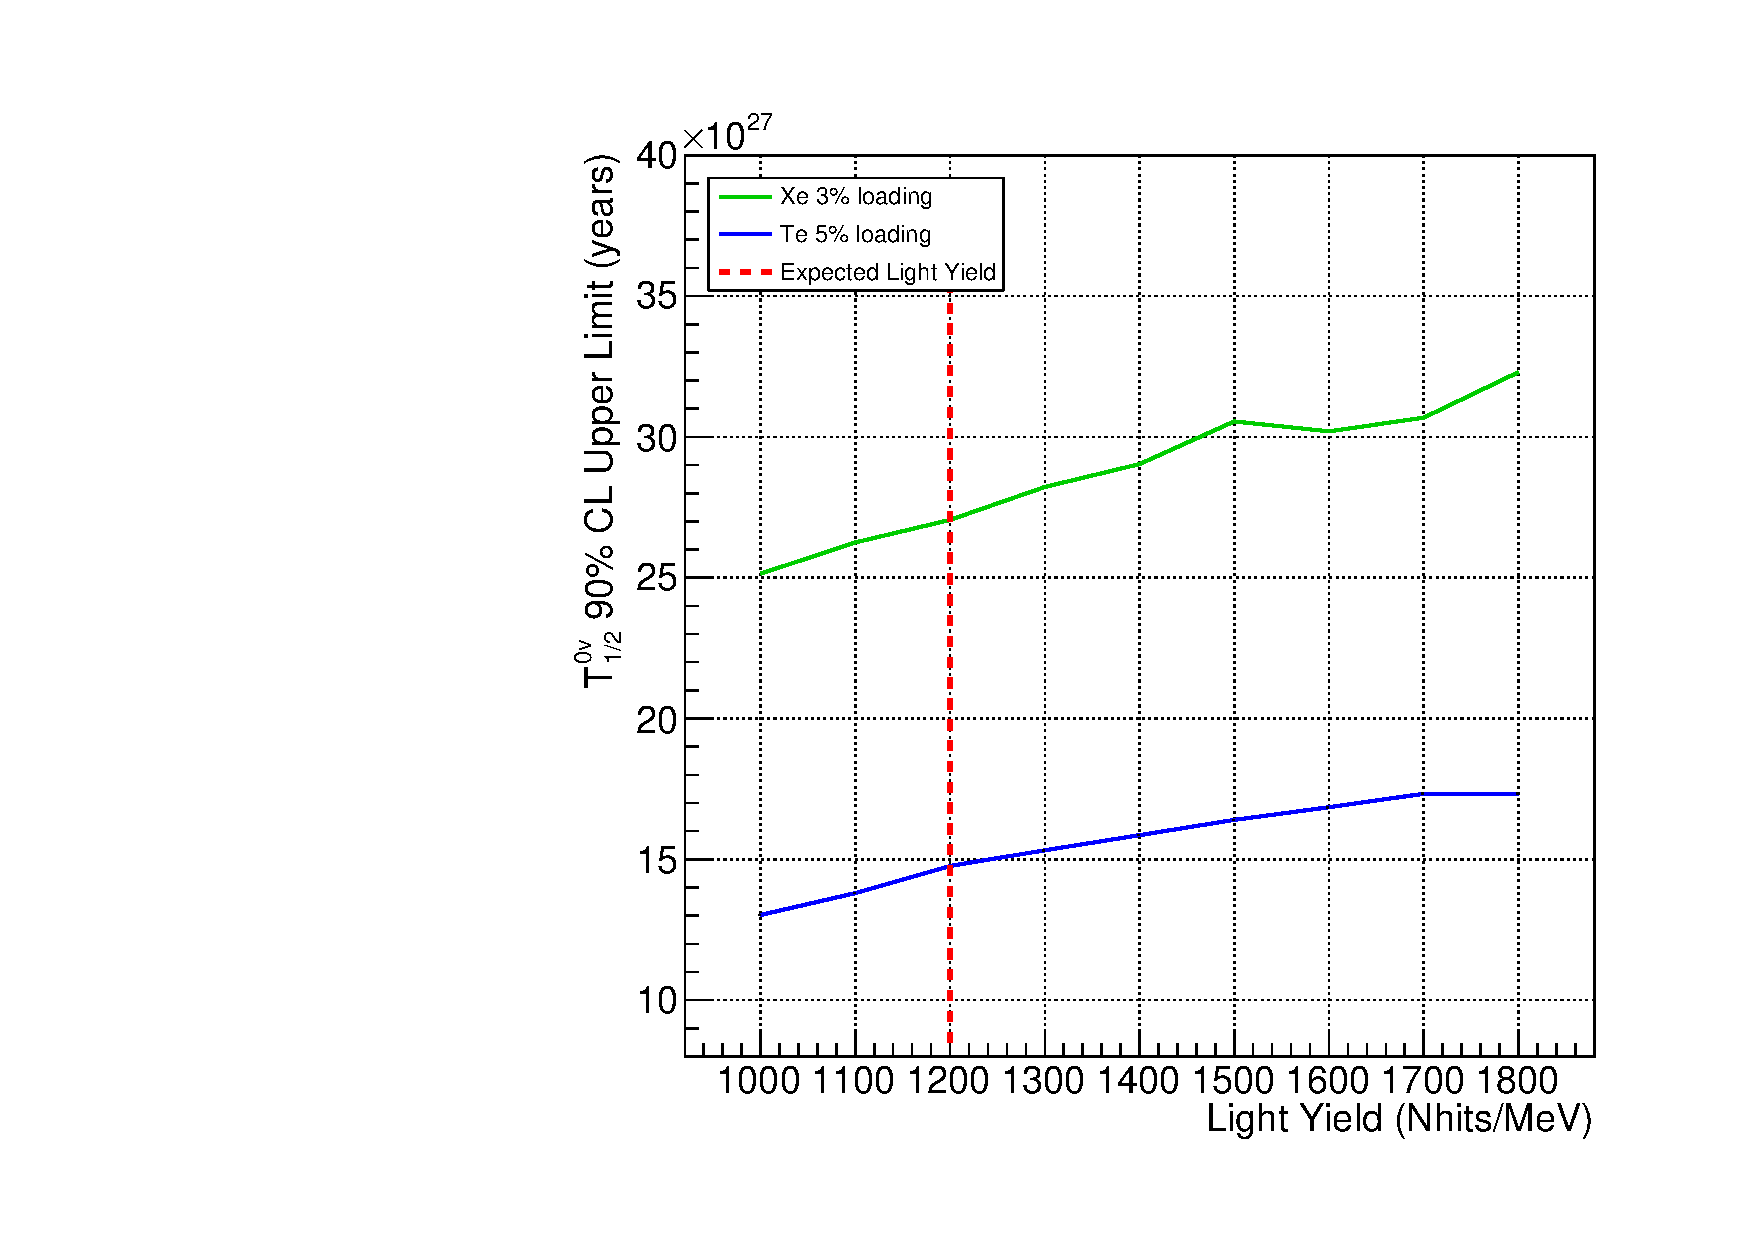
\includegraphics[width=\textwidth]{dbd/ly_fc.pdf}
 \caption{Light yield}
 \label{fig:scale-ly}
\end{subfigure}
\begin{subfigure}[b]{0.35\textwidth}
 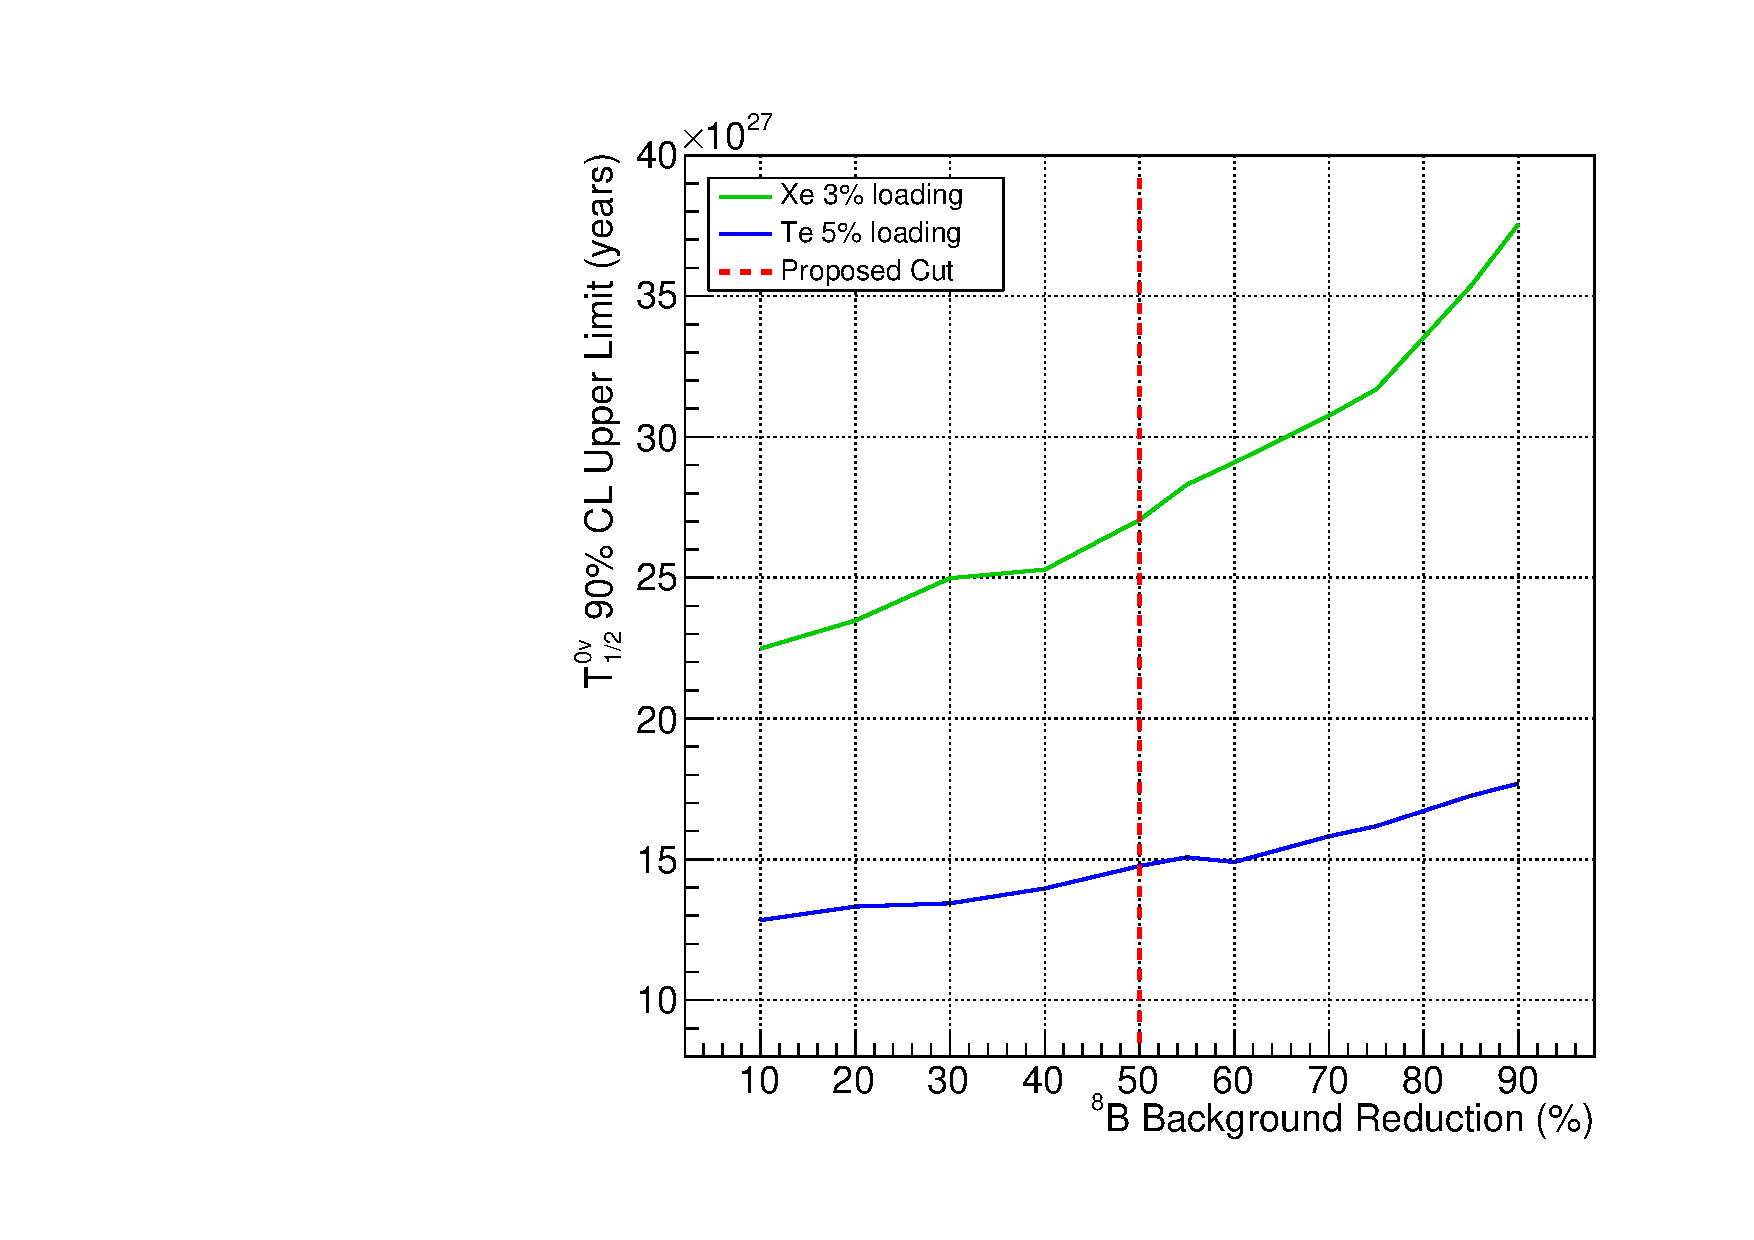
\includegraphics[width=\textwidth]{dbd/b8_reduction_fc.pdf}
 \caption{$^8$B solar neutrinos' reduction}
 \label{fig:scale-b8}
\end{subfigure}\\
%\begin{subfigure}[b]{0.33\textwidth}
% 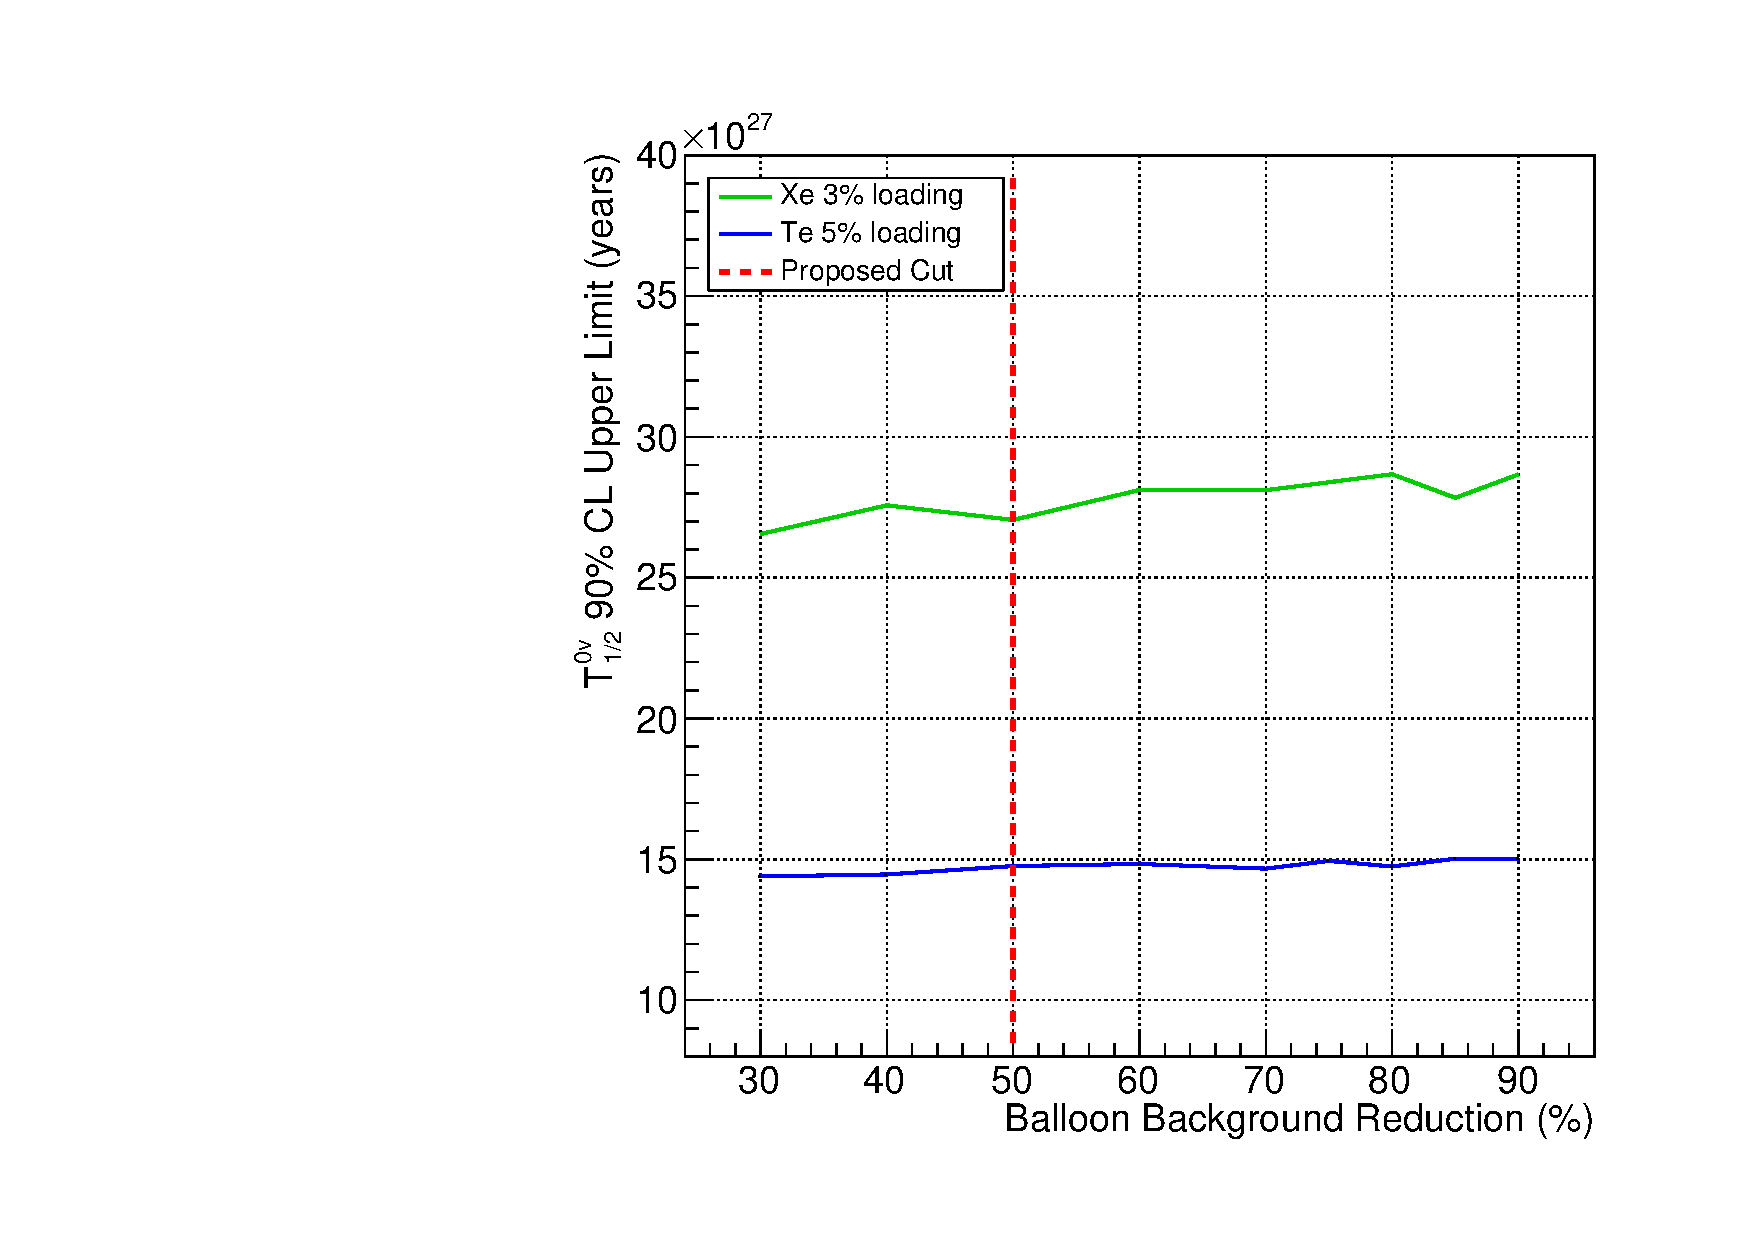
\includegraphics[width=\textwidth]{dbd/externals_reduction_fc.pdf}
% \caption{Reduction factor for external backgrounds}
% \label{fig:scale-ext}
%\end{subfigure}
%\begin{subfigure}[b]{0.35\textwidth}
% 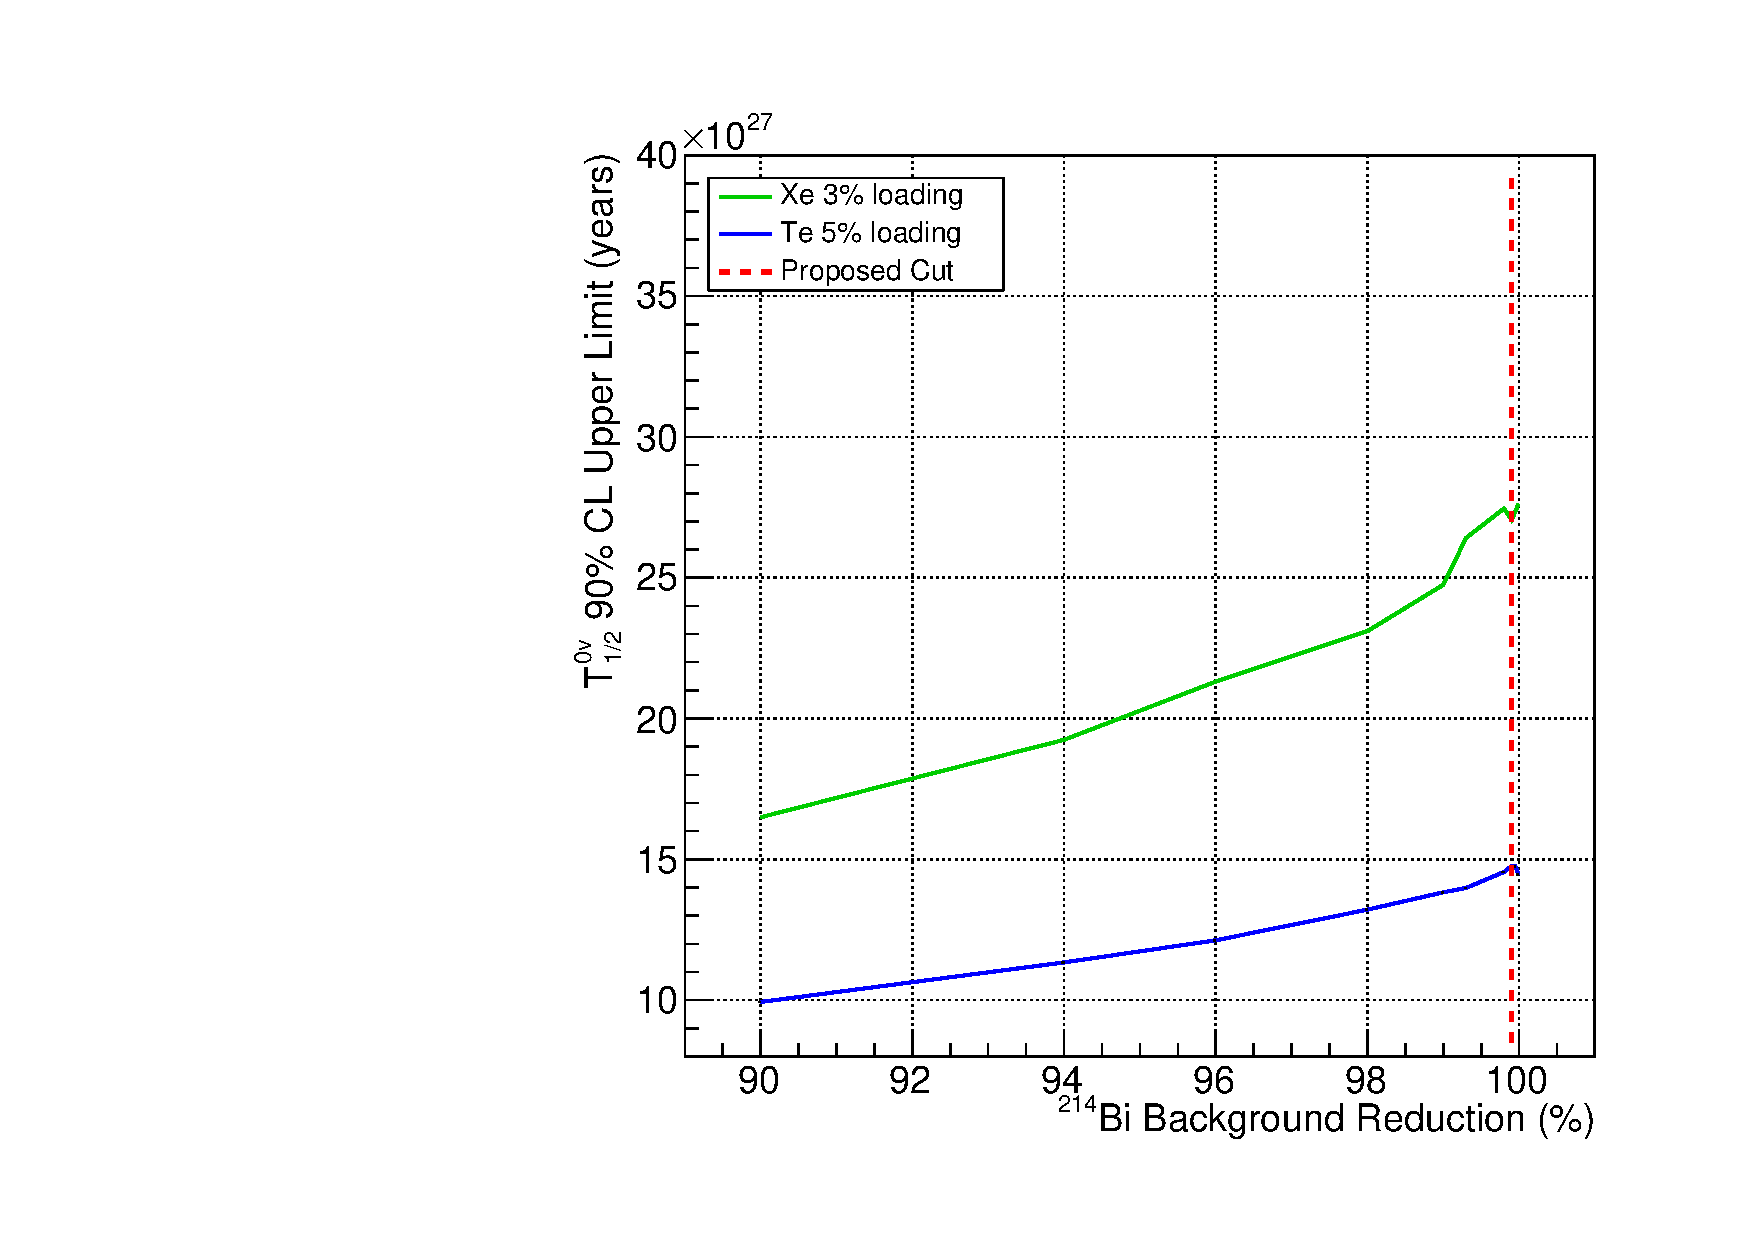
\includegraphics[width=\textwidth]{dbd/bi214_reduction_fc.pdf}
% \caption{Reduction factor for $^{214}$Bi}
% \label{fig:scale-bi214}
%\end{subfigure}
\caption{Mass sensitivity as a function of key experimental parameters. The vertical dashed red lines show the values used in the analysis.}
\label{fig:scaling-plots}
\end{figure}

\begin{figure}
\centering
\begin{subfigure}[b]{0.45\textwidth}
 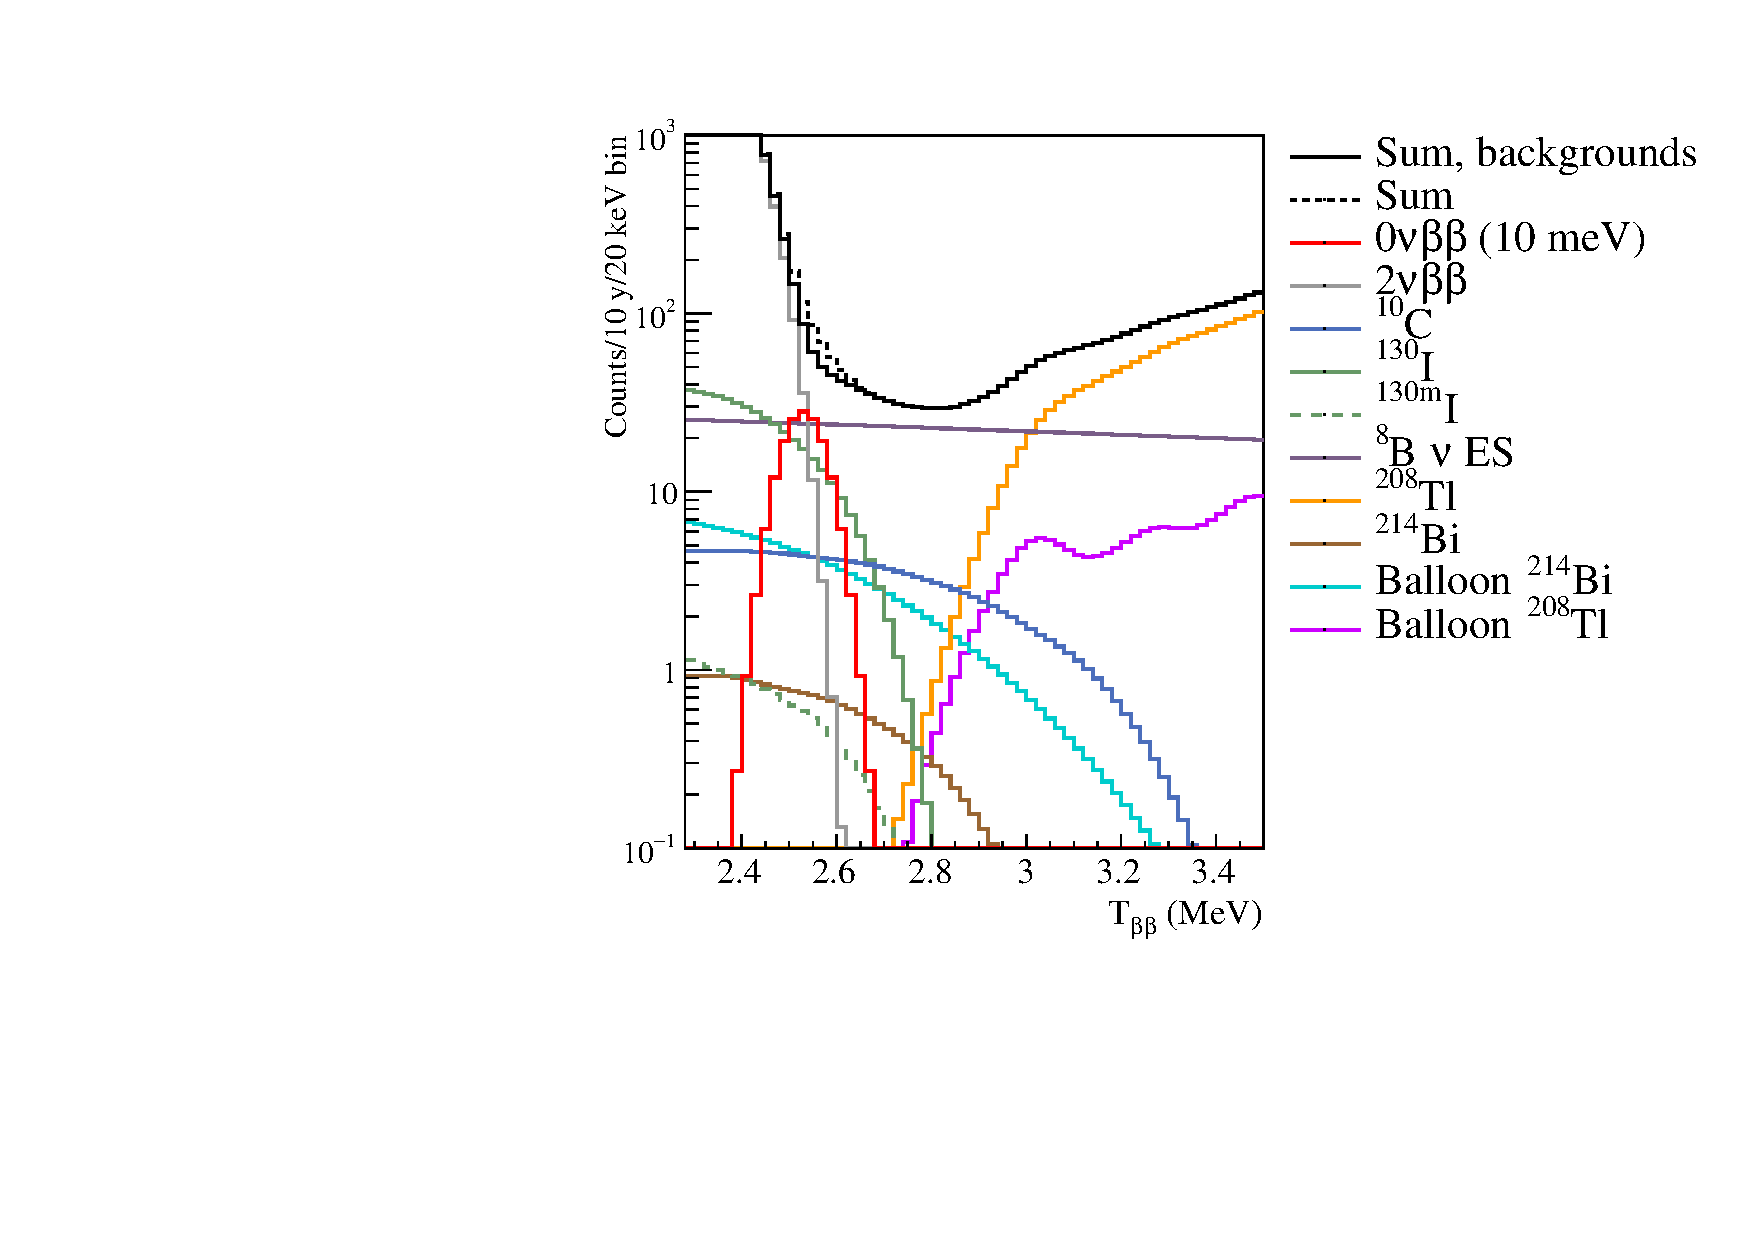
\includegraphics[width=\textwidth]{dbd/spectrum_plot_te_5.pdf}
 \caption{5\% $^{nat}$Te loading}
 \label{fig:spectrum-te}
\end{subfigure}
\begin{subfigure}[b]{0.45\textwidth}
 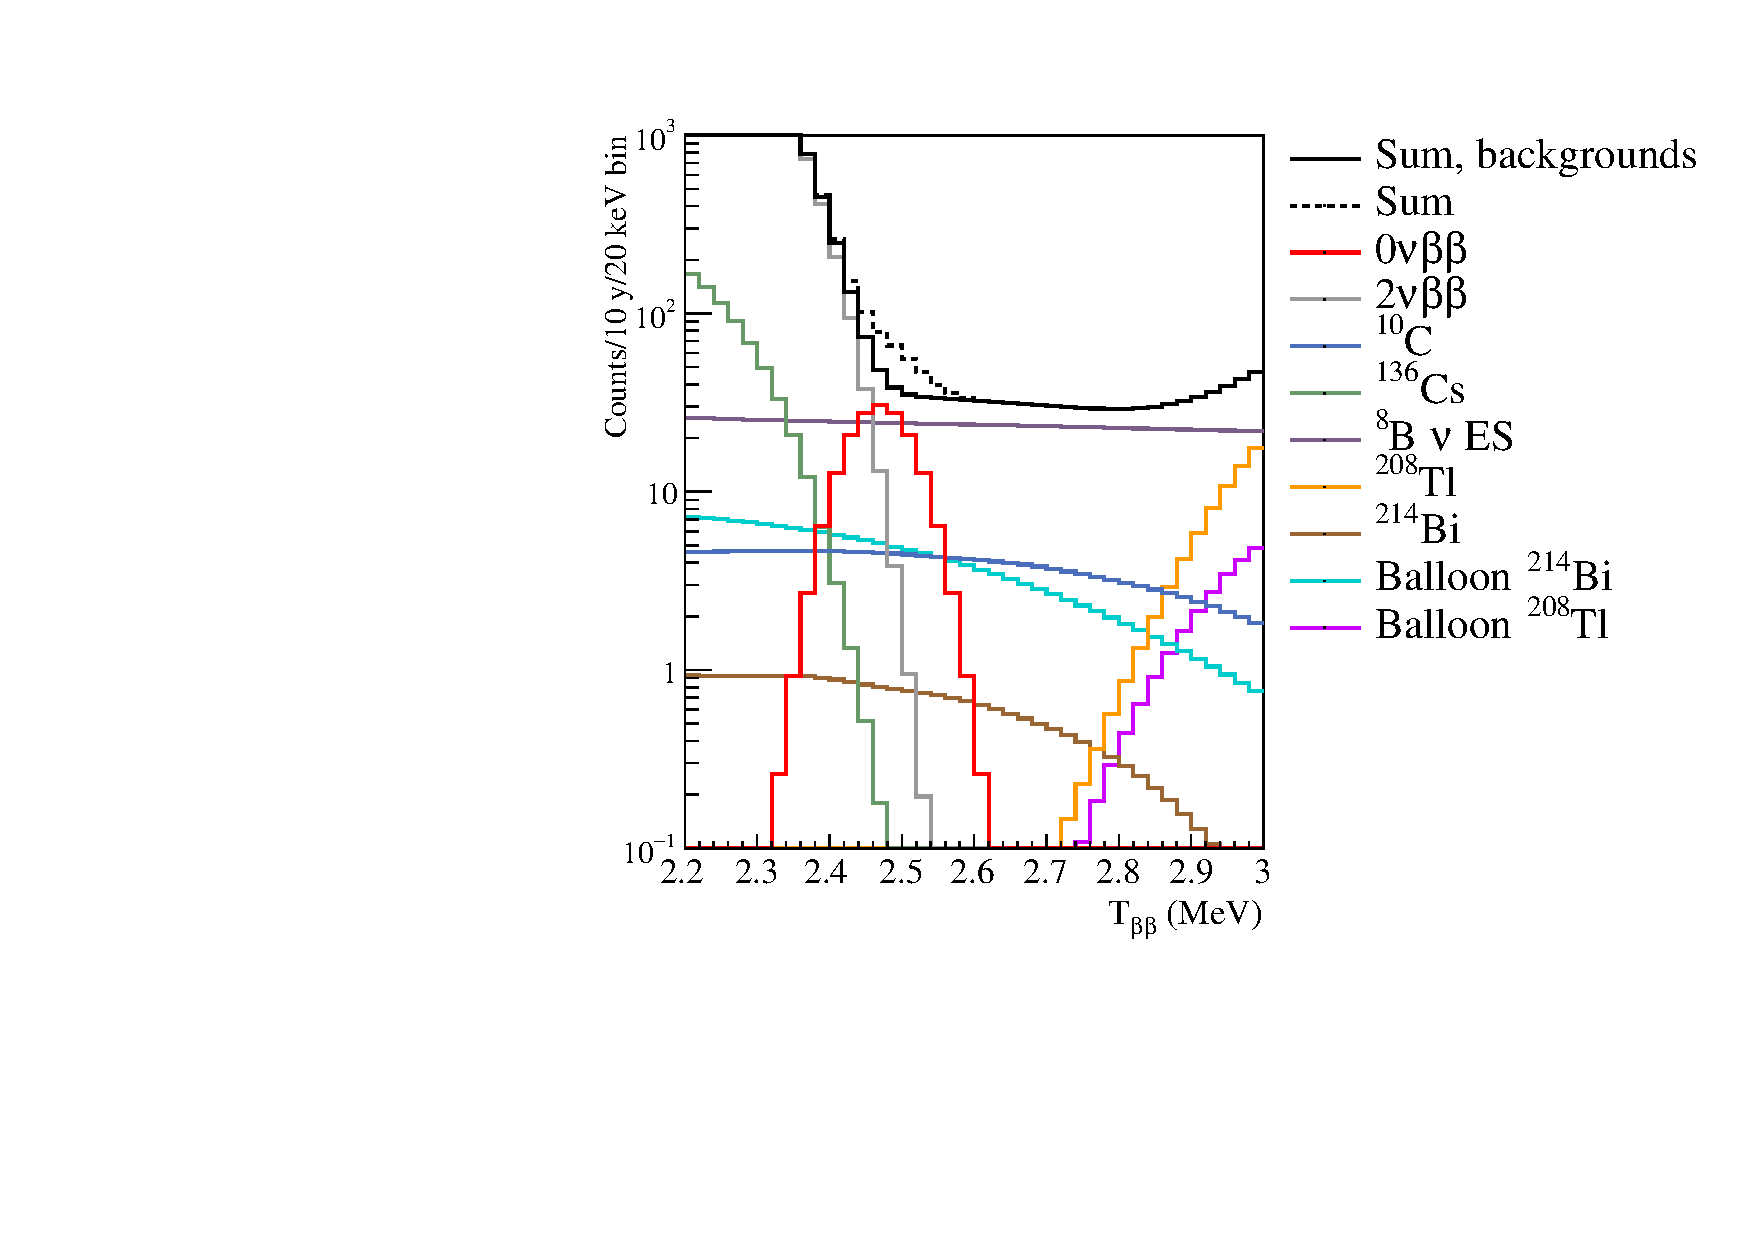
\includegraphics[width=\textwidth]{dbd/spectrum_plot_xe.pdf}
 \caption{3\% $^{enr}$Xe loading}
 \label{fig:spectrum-xe}
\end{subfigure}
\caption{Energy spectra near the NLDBD endpoint for events within the 7 m fiducial volume. A rejection factor of 92.5\% is assumed for $^{10}$C of , of 99.9\% for $^{214}$Bi, of 50\% for the balloon backgrounds, and 50\% for the $^8$B solar neutrinos.}
\label{fig:spectrum-plots}
\end{figure}

\noindent
%{\bf TODO:} Comment on prohibitive Xe costs?

\subsubsection{Alternative Isotopes}

Few alternative isotopes have been explored, which would be favorable in terms of annual abundance and costs: $^{100}$Mo, $^{82}$Se and $^{150}$Nd. A summary of the expected events in the NLDBD ROI and the corresponding limits on the half-life, and Majorana mass, is given in Table \ref{table::dbd::alternatives}. The selected loading of 2\% for Se and Nd is based on results of stability tests in table-top experiments. For Mo a loading up to 3\% seems to maintain good stability and optical properties. In case of Nd an enrichment factor of 90\% is considered, while the enrichment option for Mo and Se is considered less promising due to the smaller G$_{0\nu} M^{2}_{0\nu}$ value. The scintillator purity is kept at 10$^{-17}$g/g for both U and Th for all the mixtures, unless otherwise noted.

Among the alternatives explored, the 2\% enriched Nd cocktail is the only option providing a competitive limit on the effective Majorana neutrino mass, approaching the limit obtained with a 5\% Te loaded scintillator for high light yield.

\begin{table}
\centering
\scalebox{0.9}{
\begin{tabular}{cccc}
\toprule
                          & \multicolumn{3}{c}{\bf Events/ROI$\cdot$10 y} \\
{\bf Signal}              & $^{nat}$Se  & $^{nat}$Mo   & $^{enr}$Nd \\
\midrule
Loading fraction (\%) & 2 & 3 & 2 \\
Isotope fraction (\%) & 8.73 & 9.82 & 90 \\
Loaded isotope mass [t] & 3.2 & 5.4 & 33.2 \\
%$0\nu\beta\beta$ (10 meV) & 21.4       & 21.7 & 31.4      \\
\midrule
$2\nu\beta\beta$          & 117.3 &  325.6  & 2042     \\
$^8$B Solar ES  (50\%)           & 136.2     & 135.6 & 132.9      \\
$^{10}$C  (92.5\%)                & 9.91       & 8.49 & 0.28       \\
$^{100}$Tc \cite{eijiri14, eijiri17}                 & ---       & 0.34 & ---        \\
$^{82}$Br \cite{eijiri14, eijiri17}               & 0.21        & --- & ---        \\
$^{150}$Pm \cite{eijiri14, eijiri17}               & ---        & --- & 0.145       \\
$^{208}$Tl                & 158.4       & 198.7 & 563.4      \\
$^{214}$Bi  (99.9\%)               & 0.18        & 0.09 & --- (*)        \\
Balloon $^{214}$Bi  (50\%)       & 3.8       & 3.0 & 0.2       \\
Balloon $^{208}$Tl  (50\%)      & 31.7       & 31.0 & 50.5       \\
\midrule
{\bf Total}               & 457.8      & 702.8 & 2789.9      \\ \hline \hline
Expected T$_{1/2}$ ($\times10^{27}$ yr) & 2.2 & 2.4 & 5.1 \\
Expected mass (meV) & 15.5 & 13.8 & 7.6 \\ \hline
\bottomrule
\end{tabular}}
\caption{Expected background counts in 10 years of data taking in the ROI. In parenthesis is shown the reduction factor applied. (*) Assumed 10$^{-16}$ g/g in U. Limits on the effect Majorana neutrino mass are obtained for 90\% C.L. (FC approach) with phase space factors from \cite{2012PhRvC..85c4316K} and matrix elements from \cite{Barea:2013wb} (g$_{A}$=1.269).}
\label{table::dbd::alternatives}
\end{table}

%\begin{figure}
%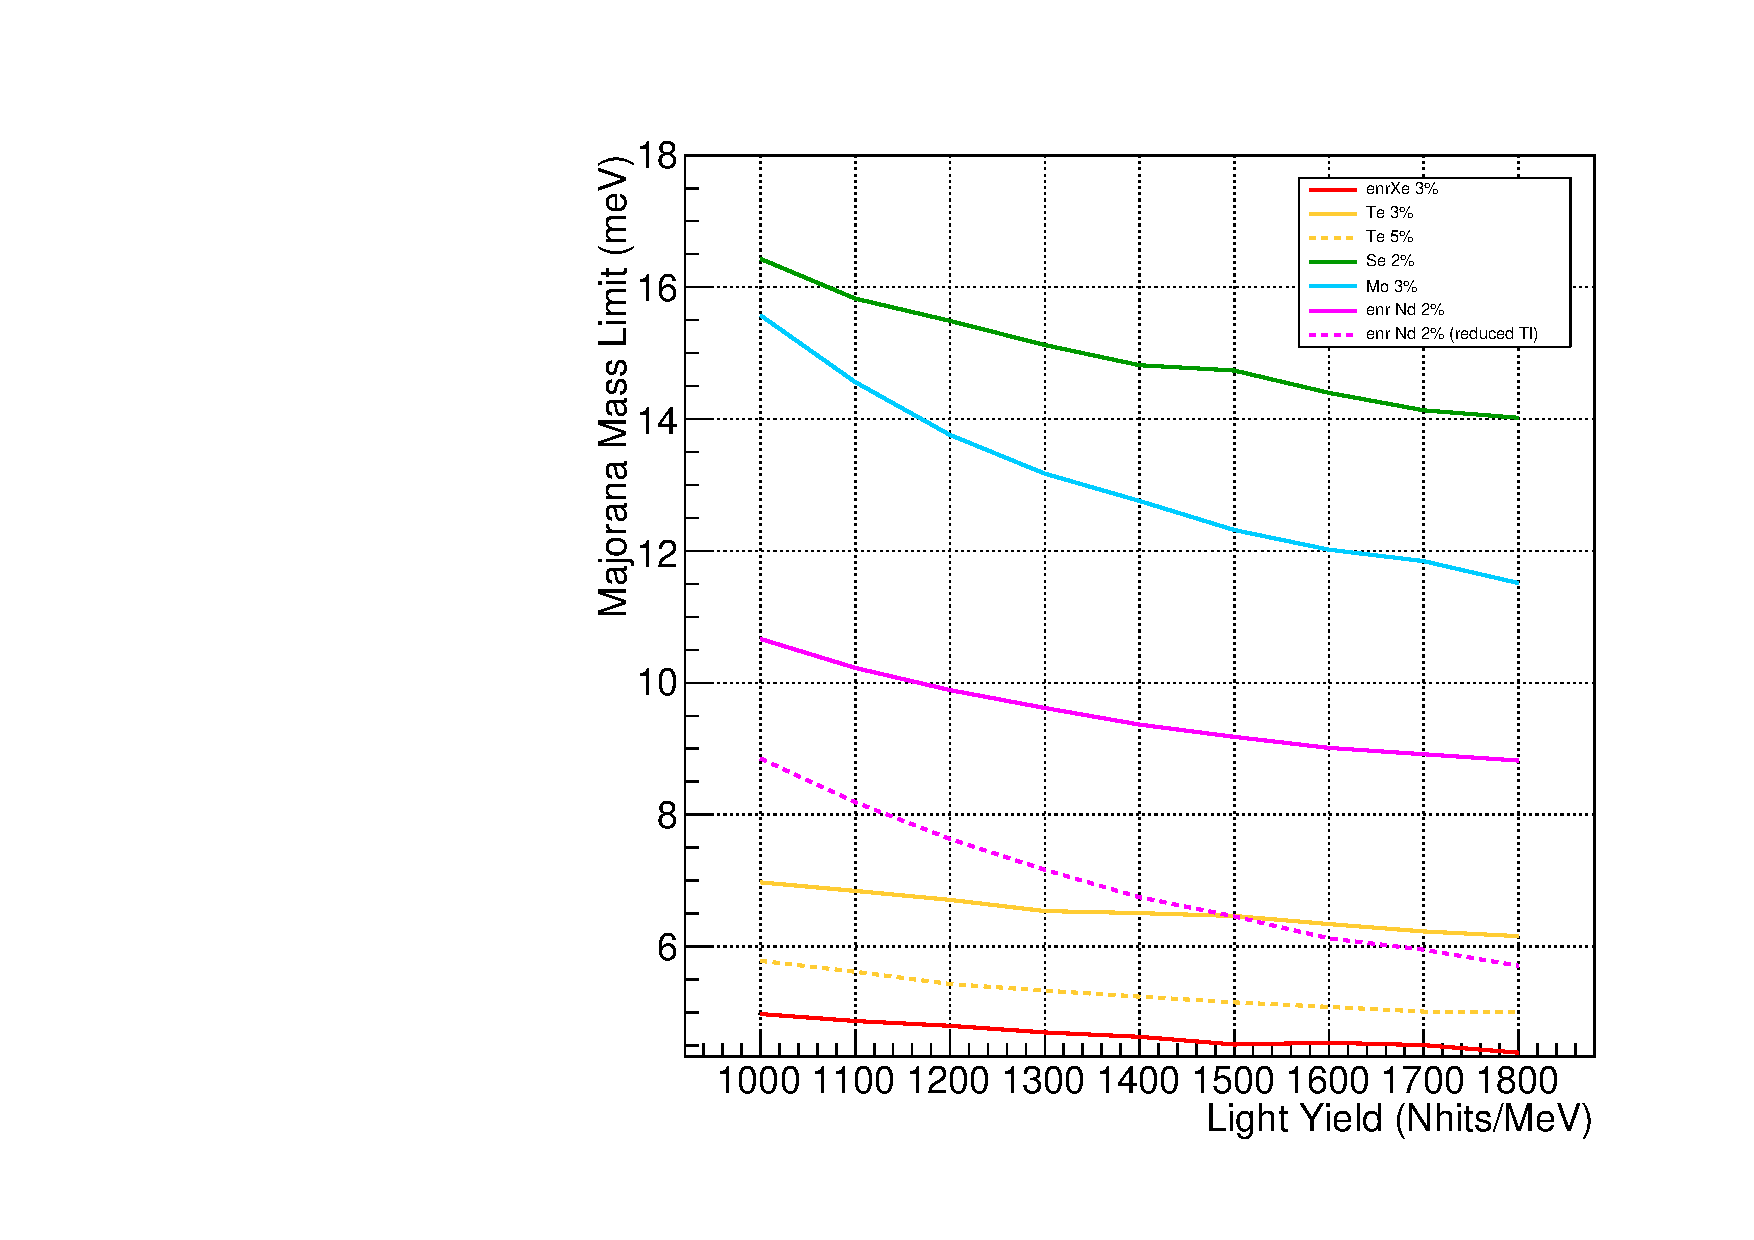
\includegraphics[scale=0.6]{dbd/ly_comparison_mass.pdf} 
%\caption{Comparison plot for various loading and isotopes. Shown is the limit on the effective Majorana neutrino mass as a function of the light yield.  3\%-$^{enr}$Xe loading still has the best limit, however 5\% Te and 2\%- $^{enr}$Nd are a competitive option. \label{fig::dbd::LY}}
%\end{figure}

%\section{Acknowledgements}
%
%\begin{thebibliography}{99}
%\bibitem{bxo16} N. Rossi, Neutrino 2016 Conference, London, 3---10 July 2016, \url{http://neutrino2016.iopconfs.org/IOP/media/uploaded/EVIOP/event_948/14.00__1_.pdf}
%\bibitem{mei09} D. M. Mei et al., Astropart. Phys. 31, 417–420 (2009).
%\bibitem{baudis15} L. Baudis et al., Eur. Phys. J. C 75, 485 (2015).
%\bibitem{zhang16} C. Zhang et al., Astropart. Phys. 84, 62--69 (2016).
%\bibitem{norm05} E. B. Norman et al., Nucl. Phys. B (Proc. Suppl.) 143, 508 (2005).
%\bibitem{bard97} D.W. Bardayan et al., Phys. Rev. C 55, 820 (1997).
%\bibitem{wang15} B.S. Wang et al., Phys. Rev. C 92, 024620 (2015).
%\bibitem{lozza15}  V. Lozza and J. Petzoldt, Astropart. Phys. 61, 62--71 (2015).
%\bibitem{snop16} S. Andringa et al., Advances in High Energy Physics 2016, 6194250 (2016).
%\bibitem{galb05} C. Galbiati, A. Pocar, D. Franco, A. Ianni, L. Cadonati, S. Schoenert, Phys.Rev. C 71 055805 (2005).
%\bibitem{gando16} Y Gando, Nuclear and Particle Physics Proceedings, vol. 273- 275, pp. 1842-1846 (2016).
%\bibitem{hagn00} T. Hagner et al., Astro. Phys. 14, 33--47, (2000).
%\bibitem{mei06} D. M. Mei and A. Hime, Phys. Rev. D 73, 053004 (2006).
%\bibitem{zbiri10} K. Zbiri, arxiv:0910.3714v3 [hep--ph] (2010).
%\bibitem{bxo2013} Borexino Collaboration, G. Bellini et al., JCAP08 49 (2013).
%\bibitem{SNO_3ph} SNO Collaboration, B. Aharmim et al., Physical Review C 88, 025501 (2013).
%\bibitem{Cuore017} C. Alduino et al., Eur. Phys. J. C 77 (2017).
%\bibitem{exo14}  J.B. Albert et al., Phys. Rev. C 89, 015502 (2014). 
%\bibitem{kam03} KamLAND Collaboration, K. Eguchi et al., Physical Review Letters 90, 021802, (2003).
%\bibitem{bxo09} Borexino Collaboration, C. Arpesella et al., Physical Review Letters 101,091302, (2008).
%\bibitem{gando13} A. Gando et al. Phys. Rev. Lett. 110, 062502 (2013).
%\bibitem{radiopurityorg} \url{https://www.radiopurity.org/rp/rp/_design/persephone/index.html?all}
%\bibitem{kamLAND_Zen} I. Shimizu, Frontiers of liquid Scintillator Technology (FroST16), March 18, 2016
%\url{https://indico.fnal.gov/getFile.py/access?contribId=45&sessionId=25&resId=0&materialId=slides&confId=10355}
%\bibitem{eijiri14} H. Ejiri and S. R. Elliott, Phys. Rev. C 89, 055501, (2014).
%\bibitem{eijiri17} H. Ejiri and S. R. Elliott, Phys. Rev. C 95, 055501 (2017).
%\bibitem{decay0} O.A.Ponkratenko, V.I.Tretyak, Yu.G.Zdesenko, Phys. At. Nucl. 63, 1282   (2000)  (nucl-ex/0104018)
%\bibitem{2012PhRvC..85c4316K} Kotila, J., \& Iachello, F. (2012). Phase-space factors for double-$\beta$ decay. Physical Review C - Nuclear Physics, 85(3), 034316. http://doi.org/10.1103/PhysRevC.85.034316
%\bibitem{Barea:2013wb} Barea, J., Kotila, J., \& Iachello, F. (2013). Nuclear matrix elements for double-$\beta$ decay. Physical Review C - Nuclear Physics, 87(1).
%\bibitem{KD-Zen} KamLAND-Zen Collaboration, Phys. Rev. Lett. 117, 082503 (2016).
%\bibitem{KZ-2011} Yoshihito Gando, Present Status of KamLAND-Zen, talk on International Workshop on Double Beta Decay and Neutrinos, Nov. 2011.
%\end{thebibliography}
%
%%\bibliographystyle{alpha}
%%\bibliography{sample}
%
%\end{document}

